\documentclass[12pt]{notes}

% Command for Questions
%\question{}

% Command for Notes
% \note{}

% Code to create a minipage where you can type in class notes. 
%%\begin{minipage}[l][2cm][c]{\textwidth}
%\begin{comment}

%\end{comment}
%%\end{minipage}

\usepackage{listings}

% In order for the minted code to run, we had to create a new compilation routine called pdflatex+shellEscape.
% This includes a --shell-escape command which should ONLY be used when pygmentized is required as it compromises security. 
% We also had to add pygmentize (a python package) to the system path (BEFORE miktex) and then restart the computer. 
\usepackage{minted}
\usemintedstyle{borland}
\lstset{language=SAS, 
  breaklines=true,  
  basicstyle=\ttfamily\bfseries,
  columns=fixed,
  keepspaces=true,
  identifierstyle=\color{blue}\ttfamily,
  keywordstyle=\color{cyan}\ttfamily,
  stringstyle=\color{purple}\ttfamily,
  commentstyle=\color{green}\ttfamily,
  } 
  
% \begin{minted}{sas}
% \end{minted}


% Begin Document
%==============================================================================
\begin{document}
% Include the Title of the Handout
\ntitle{4.1: Penalized Regression}

% Include Numbered Sections
\section{Why Penalized Regression?}

Recall linear regression model and predictive equation:
 \begin{eqnarray}
   Y & = & \beta_0 + \beta_1 X_1 + \ldots + \beta_{p-1}X_{p-1} + \varepsilon \nonumber \\
   & & \nonumber \\
   \hat{Y} & = & b_0 + b_1 X_1 + \ldots + b_{p-1}X_{p-1} \nonumber
 \end{eqnarray}
 
 \nspace
 
 IF the assumptions regarding residuals are satisfied, then ordinary least squares (OLS) provides the best (i.e. minimum variance) unbiased estimator for each $\beta_k \,(k = 1, \ldots, p-1)$ using the \textbf{loss function}
 $$\sum_{i=1}^n\left(Y_i - \hat{Y}_i\right)^2.$$
 
\nspace
\textbf{However}, when multicollinearity is present, the variance of the estimates for the $\beta_k$ are inflated.

\nspace 
\question{(Individual) What are some undesirable consequences of $\beta_k$'s with inflated variance?}

 \begin{minipage}[l][4cm][c]{\textwidth}
%\begin{comment}
\note{
\bi
\item Interpretation: the sign/magnitude of the coefficients could be misleading or non-intuitive
\item Stability: Coefficients could change drastically for small changes in the training data, which makes it hard to persuade others that the model form is correct. 
\item Variable selection: When the number of candidate explanatory variables is large, inflated variance may cause us to throw the ``best'' predictor variables out in a stepwise search. 
\ei
}
%\end{comment}
\end{minipage}

What we would like is a way to shrink the variance of our estimated coefficients, perhaps forcing some coefficients all the way to zero (i.e. variable selection). This will allow us to \textbf{stabilize} our coefficient estimates while at the same time provide an alternative approach for variable selection. 

\nspace
However, nothing in statistics comes free. Like the ``soul stone'' from the avengers series, we must sacrifice something we love in order to obtain smaller variance and a new approach for variable selection. 

\nspace
\textbf{Our Solution:} Sacrifice \textbf{unbiased} estimates of the $\beta$ coefficients in order to reduce their variance. 

\question{(Individual) What does it mean to be unbiased?}

 \begin{minipage}[l][4cm][c]{\textwidth}
%\begin{comment}
\note{$$E(b_k) = \beta_k$$
In other words, if I were to use multiple \textit{different} samples to fit my regression line, the estimated coefficients will all be different, but will all be centered around the true (and unknown) coefficients. This is important because it means that as my sample size increases, I expect to get estimates that are closer and closer to the ``truth''.}
%\end{comment}
\end{minipage}

\newpage
\question{(Individual) Why might we be OK with giving up unbiasedness in order to minimize variance?}

 \begin{minipage}[l][3cm][c]{\textwidth}
%\begin{comment}
\note{
\bi
\item Coefficients are biased to have smaller magnitude compared to the ``truth'' so we can still interpret the sign of each estimator. 
\item Biased, yet stable, estimates of the coefficients can often provide much greater predictive accuracy than an OLS model. 
\ei
}
%\end{comment}
\end{minipage}

 \begin{minipage}[l][2cm][c]{\textwidth}
%\begin{comment}
\note{
(draw example of unbiased, high variance distribution against biased, low variance distribution)
}
%\end{comment}
\end{minipage}

\section{Penalized Regression Approaches}
\textbf{Alternative Loss Functions}:
\begin{itemize}
  \item Ridge regression
  \begin{eqnarray}
      \sum_{i=1}^{n} \left( Y_i - \hat{Y}_i \right)^2 & + & \lambda \sum_{k=0}^{p-1} \left(\beta_k \right)^2 \nonumber
  \end{eqnarray}
  \item LASSO
  \begin{eqnarray}
    \sum_{i=1}^{n} \left( Y_i - \hat{Y}_i \right)^2 + \lambda \sum_{k=1}^{p-1} |\beta_k| \nonumber
  \end{eqnarray}
  \item Adaptive LASSO
  \begin{eqnarray}
    \sum_{i=1}^{n} \left( Y_i - \hat{Y}_i \right)^2 + \lambda \sum_{k=1}^{p-1} \frac{|\beta_k|}{b_k} \nonumber
  \end{eqnarray}
   \item Elastic Net
  \begin{eqnarray}
    \sum_{i=1}^{n} \left( Y_i - \hat{Y}_i \right)^2 + \lambda_1 \sum_{k=0}^{p-1} \left(\beta_k \right)^2 + \lambda_2 \sum_{k=1}^{p-1} |\beta_k| \nonumber
  \end{eqnarray}
\end{itemize}

\nspace
\bi
\item Select values of $\lambda$ that balances added bias with reduced variance. 
\item Our goal is impose the least amount of biasedness that we can in order to achieve an acceptable reduction in variance. 
\item One potential solution would be to select $\lambda$ in such a way that minimizes the cross validation error. 
\ei

\nspace
Check out \url{https://ww2.amstat.org/meetings/csp/2014/onlineprogram/handouts/T3-Handouts.pdf} for additional info on these approaches. 

\question{(Groups) Why is it critical that we \textbf{standardize} our variables prior to using any of the penalized regression techniques?}

 \begin{minipage}[l][2cm][c]{\textwidth}
%\begin{comment}
\note{The penalty terms do not respect differences in the \textbf{scale} of variables. Variables with a small range of values will be unfairly punished if we do not standardize.}
%\end{comment}
\end{minipage}

\subsection{Ridge Regression}

Recall Linear Algebra Representation of OLS Regression:
\begin{align*}
Y &= X\beta + \epsilon
b &= \left(X'X\right)^{-1}X'Y
b &\sim N(\beta, \left(X'X\right)^{-1}\sigma^2)
\end{align*}

Recall also how we can standardize our X and Y variables producing:

\vspace{-1em}
\begin{tabular}{l l}
\begin{minipage}[t]{3in}
\begin{eqnarray}
  Y^* & = & X^* \beta^* + \varepsilon \nonumber \\
  b^* & = & ( {X^*}' X^*)^{-1} {X^*}' Y^* \nonumber \\
      & = & ( r_{XX} )^{-1} r_{YX} \nonumber \\
  Cov(b^*) & = & (r_{XX})^{-1} \sigma^2 \nonumber
\end{eqnarray}
\end{minipage}
&
\begin{minipage}[t]{3in}
\begin{eqnarray}
  Y_{i}^* & = & \frac{1}{\sqrt{n-1}} \cdot \frac{Y_{i} - \bar{Y}}{\mbox{SD of } Y} \nonumber \\
  X_{k,i}^* & = & \frac{1}{\sqrt{n-1}} \cdot \frac{X_{k,i} - \bar{X}_k}{\mbox{SD of } X_k} \nonumber \\
  r_{XX} & = & \mbox{correlation matrix of $X$'s} \nonumber \\
  r_{YX} & = & \mbox{correlation vector between $Y$ and $X$'s} \nonumber
\end{eqnarray}
\end{minipage}
\end{tabular}

\nspace
\textbf{Ridge Regression} introduces a small positive biasing constant $\lambda > 0$ so that
\begin{eqnarray}
  b^R & = & ( r_{XX} + \lambda \cdot I)^{-1} r_{YX} \nonumber
\end{eqnarray}
where $I$ is the identity matrix (one's on the diagonal of the matrix and zeros elsewhere). 

\nspace
\textbf{SAS Code:}
\begin{minted}{sas}
proc reg data=<dataset> ridge=0 to <upper bound> by <step size> 
     outvif outest=<named dataset of relevant ridge output> 
     plots(only)=ridge(VIFaxis=log);
  model <model statement> / vif;
run;
\end{minted}

\nspace
Two graphical summaries to choose the ``right'' ridge parameter $c$:\\
(Note: these are guides; there is no ``optimal'' decision)
\begin{enumerate}
  \item Ridge Trace Plot
    \begin{itemize}
      \item (Need standardized data for this to be meaningful; SAS does internally)
      \item Simultaneous plot of $b^R_1, \ldots, b^R_{p-1}$ (using standardized data) for different ridge parameters $c$ (usually from 0 to 1 or 2)\\ \vspace{1em}
      \item As c increases from 0, the $b^R_k$ may fluctuate wildly and even change signs
      \item Eventually the $b^R_k$ will move slowly toward 0
    \end{itemize}
  \item VIF Plot
 \begin{itemize}
   \item Simultaneous plot of the variance inflation factor for the $p-1$ predictors for different ridge parameters
   \item As c increases from 0, the VIF drop toward 0
 \end{itemize}

\end{enumerate}

\vspace{1em}

In general, choose smallest ridge parameter $c$:
\begin{enumerate}
   \item where the $b^R_k$ first become ``stable''
   (their approach towards 0 has slowed)
   \item and the VIF's have become ``small enough''
   (close to 1 or less than 1)
\end{enumerate}

\begin{comment}
Why is it called ``ridge'' regression?
\begin{itemize}
  \item $c\lambda$ is added to diagonal of $r_{XX}$ $\rightarrow$ makes sort of ridge there
  \item ridge trace plot shows how each $b^R_k$ follows a ridge for increasing $c$
\end{itemize}
\end{comment}

\subsubsection{Comments on Ridge Regression}
\begin{itemize}
  \item Choice of ridge parameter is somewhat subjective, but must be defendable (i.e. with a trace plot)
  \item given ridge parameter $c$, can get resulting parameter estimates ${b}$ on the ``unstandardized'' (original data) scale
      \begin{itemize}
        \item SAS gives these automatically, but need textbook equation 7.46b to get intercept $b_0$:
             \begin{eqnarray}
               \beta_0 & = & \bar{Y} - \beta_1 \bar{X}_1 - \beta_2 \bar{X}_2 - \ldots - \beta_{p-1} \bar{X}_{p-1} \nonumber
             \end{eqnarray}
      \end{itemize}
  \item ridge regression estimates ${b}$ tend to be more robust against small changes to data than are OLS estimates
  \item predictors with very unstable ridge trace (tends toward zero without any plateau or slowing down) may be dropped from model, providing an alternative to stepwise variable selection techniques
\item {\bf major limitation}: traditional inference is not directly applicable to ridge regression estimates (part of our ``soul stone'' sacrifice)\\
\end{itemize}

\subsection{LASSO (Least Absolute Shrinkage and Selection Operator)}

Find $b$ to minimize
  \begin{eqnarray}
    \sum_{i=1}^{n} \left( Y_i - \hat{Y}_i \right)^2 + \lambda \sum_{k=1}^{p-1} |\beta_k| \nonumber
  \end{eqnarray}
  
 Switching from $\lambda \sum_{k=1}^{p-1} \beta_k^2$ in ridge regression to $\lambda \sum_{k=1}^{p-1} |\beta_k|$ in LASSO, may seem minor, but this change causes $b_k$ values to now shrink all the way to zero. 


\begin{figure}[H]
\centering
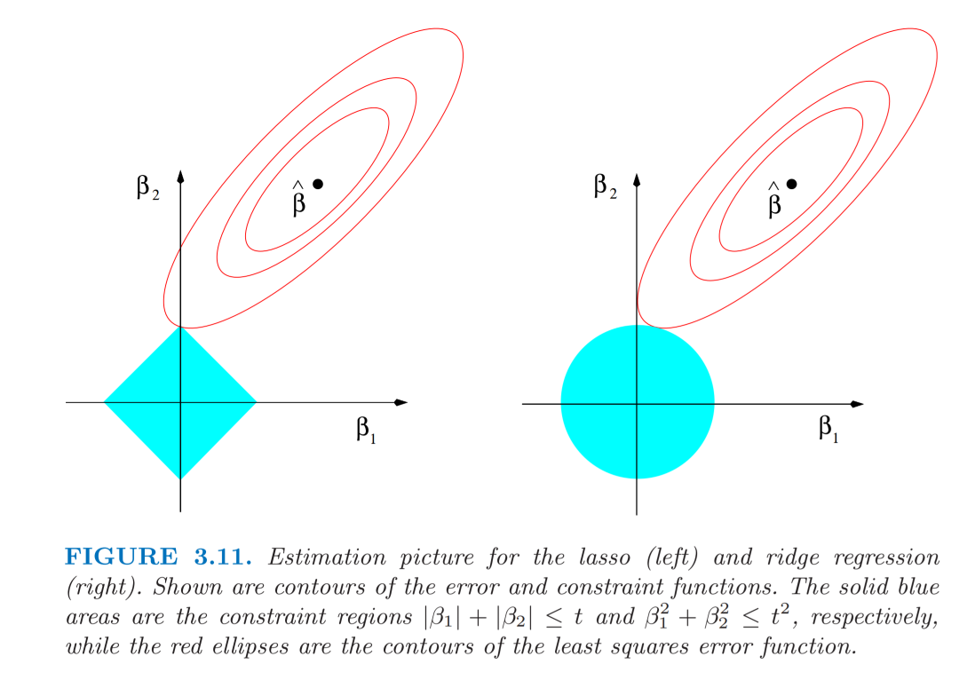
\includegraphics[width = 0.75\textwidth]{figures/module4/lasso.png}
\end{figure}

Options exist for choosing $\lambda$ \note{We can use these because we now have models with different numbers of coefficients, not the case in ridge regression.}
\begin{itemize}
  \item likelihood function-based criteria (Adj. $R^2$, $C_p$, AIC, SBC, etc.)
  \item cross-validation
    \begin{itemize}
      \item withhold some of the data, fit on the rest, then predict on withheld portion
      \item select $\lambda$ to minimize something like (others exist)
        \begin{eqnarray}
          PRESS & = & \sum_{i=1}^{n} \left( \frac{Y_i - \hat{Y}_i }{1 - h_{ii}} \right)^2 \nonumber
        \end{eqnarray}
    \end{itemize}
\end{itemize}

\nspace
\textbf{SAS Code}
\begin{minted}{sas}
proc glmselect data=<dataset> plots=(criterion <measure>);
 class <all qualitative variables>;
 model <your model>
        / selection=lasso(adaptive choose=<selection method> stop=none);
 output out=<output dataset> p=<lasso predictions>;
run;
\end{minted}


One way to visualize progress of model is to show ASE as each variable is added\\ \vspace{4em}
$$\text{ASE} = \frac{\text{SSE}}{n} \qquad MSE = \frac{\text{SSE}}{n-p}$$. 

\subsection{Adaptive LASSO}
\begin{itemize}
 \item  Problem: LASSO is known to give more biased estimates of nonzero coefficients
 \item  Solution: Allow higher penalty for zero coefficients and lower penalty for nonzero coefficients
\end{itemize}

\vspace{1em}

Find $b$ to minimize
  \begin{eqnarray}
    \sum_{i=1}^{n} \left( Y_i - \hat{Y}_i \right)^2 + \lambda \sum_{k=1}^{p-1} \frac{|\beta_k|}{b_k} \nonumber
  \end{eqnarray}

\vspace{1em}

``Adaptive'' weights: $\frac{1}{b_k}$, where $b_k$ is obtained from an initial model fit (using OLS or regular LASSO or something else) \\
-- control shrinking of zero coefficients more than nonzero coefficients\\

\subsection{Elastic Net}
\begin{quotation}
\textit{Similar to the lasso, the elastic net simultaneously does automatic variable selection and continuous shrinkage, and it can select groups of correlated variables. It is like a stretchable fishing net that retains ‘all the big fish’”} - Zou and Hastie (2005)
\end{quotation}

Some limitations of LASSO:
\begin{itemize}
  \item When number of predictors ($p-1$) exceeds sample size ($n$), LASSO will select up to $n$ predictor variables before it saturates.\\ \vspace{1em} % a problem in high-dimensional data like genomics
  \item In the presence of high multicollinearity, LASSO tends to select only one variable from the group of correlated predictors.\\ \vspace{1em} % could miss out on variable effects
  \item When sample size ($n$) exceeds number of predictors ($p-1$) \underline{and} there is high multicollinearity, LASSO is out-performed (prediction-wise) by ridge regression.
\end{itemize}

\nspace

Elastic Net overcomes these limitations: % best of ridge regression \underline{and} LASSO
\begin{itemize}
  \item can select more than $n$ variables
  \item can select more than one variable from a group of highly collinear predictors
  \item can achieve better predictive performance % and in general should never do worse than lasso or ridge
\end{itemize}

\nspace

Find $b$ to minimize
  \begin{eqnarray}
    \sum_{i=1}^{n} \left( Y_i - \hat{Y}_i \right)^2 + \lambda_1 \sum_{k=0}^{p-1} \left(\beta_k \right)^2 + \lambda_2 \sum_{k=1}^{p-1} |\beta_k| \nonumber
  \end{eqnarray}
  
\question{(Groups) Which of the following is NOT a good scenario to used penalized regression techniques? Why?
\begin{enumerate}
\item Facebook is trying to create a model to predict the likelihood of a user responding positively to a certain type of ad. 
\item The Huntsman Cancer institute is trying to determine which active genes in a person’s DNA increase the likelihood of Pancreatic cancer. 
\item The USU Agriculture Experiment Station is trying to determine if a change in the composition of feed significantly influences the milk output of dairy cows.
\end{enumerate}
}

\begin{minipage}[l][4cm][c]{\textwidth}
%\begin{comment}
\note{
\textbf{3} is the correct answer because:
\bi 
\item This scenario is an experiment rather than an observational study. 
\item We are interested in the significance of an effect, rather than accurate predictions. 
\ei
}
%\end{comment}
\end{minipage}



% End the Document
%==============================================================================
\end{document}